\documentclass[10pt]{article}
\usepackage[margin=0.78in]{geometry}
\usepackage{amsmath,amssymb,amsthm,mathtools,bm}
\usepackage{booktabs,array,enumitem,microtype,placeins}
\usepackage{graphicx,subcaption}
\graphicspath{{../../}{./}}
\usepackage{xcolor}
\usepackage{hyperref}
\usepackage{tikz}
\usetikzlibrary{arrows.meta,positioning,fit,backgrounds}

\hypersetup{colorlinks=true,linkcolor=blue!55!black,citecolor=blue!55!black,urlcolor=blue!55!black}
\setlist{nosep,leftmargin=1.6em}
\newtheorem{theorem}{Theorem}[section]
\newtheorem{proposition}[theorem]{Proposition}
\newtheorem{lemma}[theorem]{Lemma}
\newtheorem{corollary}[theorem]{Corollary}
\newtheorem{assumption}[theorem]{Assumption}
\theoremstyle{definition}
\newtheorem{definition}[theorem]{Definition}
\newtheorem{example}[theorem]{Example}
\theoremstyle{remark}
\newtheorem{remark}[theorem]{Remark}

\newcommand{\E}{\mathbb E}
\newcommand{\Pp}{\mathbb P}
\newcommand{\R}{\mathbb R}
\newcommand{\Sph}{\mathbb S}
\newcommand{\norm}[1]{\left\lVert#1\right\rVert}
\newcommand{\abs}[1]{\left|#1\right|}
\newcommand{\Id}{\mathbf I}
\newcommand{\uvec}{\mathbf u}
\newcommand{\vvec}{\mathbf v}
\newcommand{\svec}{\mathbf s}
\newcommand{\Hvec}{\mathbf H}
\newcommand{\Avec}{\mathbf A}
\newcommand{\xivec}{\boldsymbol\xi}
\newcommand{\ind}{\mathbf 1}

\title{From Post-Harmonic Instability to Distributional Shape:\\
Loss-Level Conditions for Discrete Stochastic Self-Stabilization}
\author{Technical research draft}
\date{August 2026}

\begin{document}
\maketitle

\begin{abstract}
Local mini-batch SGD is governed by a random matrix product, but a local
instability threshold alone does not determine the shape of the iterates.
We give a discrete-time condition stack that separates five conclusions:
post-harmonic repulsion, nonlinear confinement, regular return to the local
region, central depletion, and spatial bimodality.  When the negative
pressure is finite and strictly convex through $q=-1$ and has a nonzero root
$k(-\alpha)=1$, post-harmonicity $k(-1)<1$ is equivalent to $\alpha>1$.
If the nonlinear SGD map also satisfies an outer Foster drift
and a regenerative return condition, the ideal zero-core radial law obeys
$\Pp(\norm{\uvec}\le r)\sim Cr^\alpha$; at fixed additive noise this is an
intermediate-window prediction requiring a uniform renewal limit.  In more than one dimension this
does not automatically imply a dip in every coordinate: a fixed projection
inherits the exponent only under angular pinning or an equivalent
inverse-angle integrability condition.  One sufficient route to exactly two
symmetric lobes additionally assumes reflection symmetry and excludes
competing modes; a noisy flip interpretation further requires sign reversal
and two-step contraction.  We instantiate
the theory in (i) exact random-covariate linear regression with a smooth
asymptotically linear higher-order completion having bounded outer remainder
and (ii) a curvature-changing model whose mixed third
derivative lowers sharpness after escape.  Exact discrete simulations test
the separate mechanisms and include counterexamples to missing implications.
No diffusion approximation is used.
\end{abstract}

\section{Introduction}

The deterministic edge of stability is often described by a Hessian
eigenvalue reaching $2/\eta$.  Under mini-batch SGD, however, the local
multiplier is a random matrix $\Id-\eta\Hvec_B$, so positive moments,
typical products, and inverse moments generally cross their stability
boundaries at different step sizes.  This already makes the phrase
\emph{the stochastic edge} ambiguous on a quadratic loss.  Beyond the local
edge, the quadratic model is more seriously incomplete: it predicts escape
and cannot explain why nonlinear training remains bounded.

This paper separates the local instability diagnostic from the nonlinear
mechanisms that determine the stationary shape.  The harmonic or fractional
negative-moment condition controls how rarely a local random product returns
toward the solution.  It does not itself produce an invariant law.  A
higher-order loss must first confine large excursions and return them to the
local region.  Even then, a depleted radius need not create a dip in a fixed
neural coordinate, and a dip need not create exactly two modes.  Those
conclusions require progressively stronger angular and global-shape
conditions.

Our contributions are fourfold.  First, we give exact finite-time and
regenerative interpretations of the negative-moment edge.  Second, we state
checkable finite-step Foster, minorization, return, and angular conditions
that separate recurrence, radial depletion, directional depletion, spatial
bimodality, and phase-alternating bimodality.  Third, we extend the affine
matrix Kesten baseline with exact higher-order random-regression losses and
give a distinct smooth third-derivative model in which excursions lower a
moving sharpness coordinate.  Fourth, exact discrete experiments probe the
separate mechanisms and expose failed implications, including full-rank
random covariates, noncommuting
matrices with matched spectra, and frozen-checkpoint neural gain and cycle
probes.  We use no diffusion approximation.

\section{Question and claim hierarchy}

Let $\Phi_B$ denote one exact mini-batch SGD step and let the origin be the
reference solution.  Near the origin,
\begin{equation}
  \uvec_{t+1}=\Avec_{B_t}\uvec_t+\eta\xivec_{B_t}+\mathbf N_{B_t}(\uvec_t),
  \qquad \Avec_B=\Id-\eta\Hvec_B,
  \qquad \norm{\mathbf N_B(\uvec)}=o(\norm{\uvec}).
  \label{eq:local-map}
\end{equation}
The matrix product determines local growth.  The nonlinear term determines
whether trajectories return, which directions they occupy, and what global
shape is possible.  These roles must not be collapsed into one threshold.

\begin{figure}[htbp]
\centering
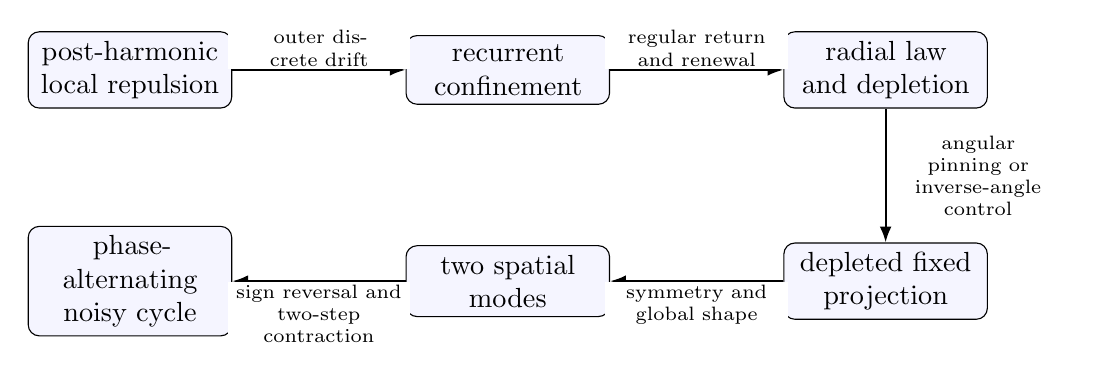
\begin{tikzpicture}[
  node distance=17mm and 22mm,
  box/.style={draw,rounded corners,align=center,minimum height=8mm,
              text width=2.35cm,fill=blue!4},
  req/.style={font=\scriptsize,align=center,text width=2.25cm,
              fill=white,inner sep=1pt},
  arr/.style={-{Latex[length=2mm]},thick}
]
\node[box] (rep) {post-harmonic\\local repulsion};
\node[box,right=of rep] (conf) {recurrent\\confinement};
\node[box,right=of conf] (rad) {radial law\\and depletion};
\node[box,below=of rad] (dep) {depleted fixed\\projection};
\node[box,left=of dep] (bi) {two spatial\\modes};
\node[box,left=of bi] (flip) {phase-alternating\\noisy cycle};
\draw[arr] (rep)-- node[req,above]{outer discrete drift} (conf);
\draw[arr] (conf)-- node[req,above]{regular return\\and renewal} (rad);
\draw[arr] (rad)-- node[req,right]{angular pinning or\\inverse-angle control} (dep);
\draw[arr] (dep)-- node[req,below]{symmetry and\\global shape} (bi);
\draw[arr] (bi)-- node[req,below]{sign reversal and\\two-step contraction} (flip);
\end{tikzpicture}
\caption{Every arrow needs a distinct hypothesis.  Harmonic instability is a
local condition; it is not, by itself, a recurrence or bimodality theorem.}
\label{fig:ladder}
\end{figure}

\begin{definition}[Three different shape statements]
For a stationary vector $\mathbf U$ and a fixed unit vector $\vvec$:
\begin{enumerate}[label=(\roman*)]
  \item \emph{radial depletion} means that the one-dimensional density of
  $R=\norm{\mathbf U}$ vanishes at $0$;
  \item \emph{directional depletion} means that the density of
  $\vvec^\top\mathbf U$ has a strict local minimum at $0$;
  \item \emph{spatial bimodality} means that this projected density has
  exactly two resolved maxima and no competing maximum.
\end{enumerate}
None of these statements is equivalent in general dimension.
\end{definition}

\begin{table}[t]
\centering
\small
\begin{tabular}{p{0.21\linewidth}p{0.34\linewidth}p{0.36\linewidth}}
\toprule
Conclusion & Main condition & What it does \emph{not} imply \\
\midrule
Local repulsion & $k(-a)<1$ for some $a>0$ & recurrence or a stationary law \\
Confinement & block Foster drift for the outer map & a density or a central dip \\
Radial depletion & root $k(-\alpha)=1$ with $\alpha>1$, regular regeneration, and renewal density & depletion of every coordinate \\
Ambient-density depletion & radial exponent $\alpha>d$ and regular angular density & directional modes \\
Directional depletion & radial law plus angular pinning/integrability & exactly two modes \\
Spatial bimodality & even density, central minimum, one positive critical point & parity-alternating dynamics \\
Noisy two-cycle & sign reversal, two-step contraction, noise below separation & a universal property of SGD \\
\bottomrule
\end{tabular}
\caption{Claim--assumption map used throughout the paper.}
\label{tab:claims}
\end{table}

\section{Local post-harmonic dynamics}

For invertible i.i.d. matrices $\Avec_n$, define on projective space
\begin{equation}
 (\mathcal P_q f)([\svec])=
 \E\!\left[\norm{\Avec_1\svec}^{q}
 f\!\left([\Avec_1\svec]\right)\right],
 \qquad \Lambda(q)=\log\rho(\mathcal P_q).
 \label{eq:transfer}
\end{equation}
We assume the projective chain has a spectral gap on a H\"older space,
$\mathcal P_q$ has a simple positive leading eigenvalue on the required
interval, and the usual moment and non-arithmetic hypotheses hold.  Then
$\Lambda'(0)=\gamma$, the top Lyapunov exponent.  In the scalar case this is
simply $\Lambda(q)=\log\E G^q$ for $G=|1-\eta h|$.

\begin{proposition}[Lyapunov--harmonic ordering]
\label{prop:harmonic-order}
Suppose $\Lambda(0)=0$, $\Lambda'(0)=\gamma>0$, and $\Lambda$ is finite and
strictly convex on $[-s_*,0]$ for some $s_*>1$.  If the nonzero negative root
$\Lambda(-\alpha)=0$ exists in this domain, then $\alpha\in(0,s_*]$ and
\begin{equation}
 \Lambda(-1)>0\Longleftrightarrow0<\alpha<1,
 \qquad \Lambda(-1)=0\Longleftrightarrow\alpha=1,
 \qquad \Lambda(-1)<0\Longleftrightarrow\alpha>1.
 \label{eq:harmonic-order}
\end{equation}
Thus ``post-harmonic'' means $k(-1)=e^{\Lambda(-1)}<1$, equivalently
$\alpha>1$, within this pressure domain.
\end{proposition}

\begin{proof}
Strict convexity, $\Lambda(0)=0$, and $\Lambda'(0)>0$ imply that
$s\mapsto\Lambda(-s)$ initially decreases below zero and can cross zero at
most once on $(0,s_*]$.  Comparing its value at $s=1$ with zero locates the
crossing on the left of, at, or on the right of one.
\end{proof}

The proposition is a statement about the local product.  It becomes a
statement about a stationary density only after the chain is shown to return
from finite amplitude.

\begin{remark}[When the literal harmonic moment exists]
For a finite discrete curvature law,
$\E|1-\eta h|^{-1}<\infty$ exactly when no atom has $h=1/\eta$.
An exact zero-gain event makes every negative moment infinite.  If instead
$h$ has a continuous density positive near $1/\eta$, then the scalar gain
$G=|1-\eta h|$ has positive density near zero:
$\E G^{-\alpha}<\infty$ for $0<\alpha<1$ but diverges for
$\alpha\ge1$.  In that case divergence at $\alpha=1$ is not evidence of
post-harmonicity; the literal criterion is undefined.  Fractional negative
moments, truncated moments $\E[(G\vee\delta)^{-\alpha}]$, and small-gain
probabilities $\Pp(G\le\delta)$ should be reported instead.  Only the
untruncated finite moments obey the exact product-pressure identity.
\end{remark}

\begin{proposition}[Finite-time anti-return bound]
\label{prop:anti-return}
For the scalar product $x_n=x_0\prod_{j=1}^nG_j$, if
$r_a=\E G^{-a}<1$ for some $a>0$, then for every $\varepsilon>0$,
\begin{equation}
 \Pp(|x_n|\le\varepsilon\mid x_0)
 \le \left(\frac{\varepsilon}{|x_0|}\right)^a r_a^n,
 \qquad
 \Pp\!\left(\min_{1\le n\le T}|x_n|\le\varepsilon\mid x_0\right)
 \le \left(\frac{\varepsilon}{|x_0|}\right)^a
 \frac{r_a}{1-r_a}.
 \label{eq:anti-return}
\end{equation}
For a matrix product the same conclusion holds, up to a uniform multiplicative
constant, whenever the negative transfer operator has spectral radius below
one and its eigenfunction is bounded above and away from zero.
\end{proposition}

\begin{proof}
Apply Markov's inequality to $|x_n|^{-a}$ and use independence; then use the
union bound and sum the geometric series.  The matrix statement follows by
the corresponding transfer-operator bound on
$\E\norm{\Avec_n\cdots\Avec_1\svec}^{-a}$.
\end{proof}

This is the precise meaning of local repulsion: a trajectory already outside
an $\varepsilon$-ball is exponentially unlikely to be carried back by the
linear product during a prescribed finite window.  It still says nothing
about what the nonlinear map does after a large excursion.

\section{Confinement and regular return}

\subsection{Exact discrete confinement conditions}

The most direct condition is stated on the finite SGD step itself.  Write
$\uvec_{t+1}=\uvec_t-\eta\mathbf g_{B_t}(\uvec_t)$, where
$\mathbf g_B=\nabla L_B$.

\begin{theorem}[One-step loss-level Foster drift]
\label{thm:loss-drift}
Suppose $PV$ is finite and locally bounded for
$V(\uvec)=1+\norm{\uvec}^2$, and there are $c\in(0,1)$ and finite $C,R$
such that, for every
$\norm{\uvec}\ge R$,
\begin{equation}
 \E\!\left[2\eta\langle\uvec,\mathbf g_B(\uvec)\rangle
 -\eta^2\norm{\mathbf g_B(\uvec)}^2\right]
 \ge c\norm{\uvec}^2-C.
 \label{eq:loss-drift}
\end{equation}
Then $V(\uvec)=1+\norm{\uvec}^2$ satisfies
$PV\le(1-c)V+C'$ outside a compact set.  A Feller chain therefore has an
invariant probability measure.  If a compact sublevel set is accessible and
small and the chain is irreducible and aperiodic, the invariant law is unique
and the chain is positive Harris recurrent.
\end{theorem}

\begin{proof}
Use the exact identity
$\norm{\uvec-\eta\mathbf g_B(\uvec)}^2=\norm{\uvec}^2
-2\eta\langle\uvec,\mathbf g_B(\uvec)\rangle
+\eta^2\norm{\mathbf g_B(\uvec)}^2$ and take conditional expectation.
The remaining conclusions are the standard discrete-time
Foster--Lyapunov/Harris implications.  No continuous-time approximation is
involved.
\end{proof}

Condition~\eqref{eq:loss-drift} shows why loss coercivity alone is not
enough: the term $\eta^2\norm{\mathbf g_B}^2$ is the exact finite-step
overshoot penalty.  A convenient alternative applies when the outer map is
asymptotically linear.

Assume that outside the local region the exact update can be decomposed as
$\Phi_B(\uvec)=\Avec_{\infty,B}\uvec+\mathbf b_B(\uvec)$, and that its
$p$th update moment is locally bounded.  By modifying $\mathbf b_B$ on the
compact inner region, use the same decomposition globally.

\begin{theorem}[Outer-cocycle confinement]
\label{thm:outer-drift}
Suppose that for some $p\in(0,1]$, integer $m\ge1$, and $\rho<1$,
\begin{equation}
 \E\norm{\Avec_{\infty,B_{m-1}}\cdots\Avec_{\infty,B_0}}^p\le\rho,
 \qquad
 \E\norm{\Avec_{\infty,B}}^p<\infty,
 \qquad
 \E\sup_{\uvec}\norm{\mathbf b_B(\uvec)}^p<\infty.
 \label{eq:outer-block}
\end{equation}
Then $V(\uvec)=1+\norm{\uvec}^p$ satisfies
$P^mV(\uvec)\le\rho V(\uvec)+C$.  If the chain is Feller, it has an
invariant probability measure.  If it is also irreducible and aperiodic and
compact sets are petite, the invariant law is unique and the chain is
positive Harris recurrent.
\end{theorem}

\begin{proof}
Iterate the decomposition for $m$ steps.  Since $p\le1$,
$\norm{\sum_j\mathbf z_j}^p\le\sum_j\norm{\mathbf z_j}^p$.  The block
product gives the coefficient $\rho$ on $\norm{\uvec}^p$, while all bounded
remainders form the constant $C$.  Tightness and the stated Harris conclusions
follow from the standard discrete-time Foster--Lyapunov theorem.
\end{proof}

The partial-product moments needed for the bounded terms inside an $m$-step
block follow from the displayed one-step moment.

\subsection{When exact regression noise verifies the kernel assumptions}

\begin{lemma}[A regression minorization]
\label{lem:regression-minorization}
Let $b\ge d$, and let a batch have $\mathbf X_B\in\R^{b\times d}$ with a
density positive on a neighborhood of a full-column-rank matrix.  Let the regression residual
$\boldsymbol\varepsilon_B$ be independent Gaussian noise with nonzero
variance.  Then
$\xivec_B=b^{-1}\mathbf X_B^\top\boldsymbol\varepsilon_B$ has, conditional
on such an $\mathbf X_B$, a nondegenerate Gaussian density.  For every compact
state set, the exact SGD transition kernel therefore minorizes a nonzero
Lebesgue measure on some ball.  If this common small set is accessible from
every state, the chain is Lebesgue-irreducible and compact sets are petite.
If the minorizing measure also charges the small set, the chain is aperiodic.
\end{lemma}

\begin{proof}
Conditional on $\mathbf X_B$, the covariance is
$\operatorname{Var}(\xivec_B\mid\mathbf X_B)=
\sigma^2b^{-2}\mathbf X_B^\top\mathbf X_B\succ0$.  On a sufficiently small
neighborhood of the chosen full-rank matrix, its smallest eigenvalue is
uniformly positive.  Continuity of the deterministic update and positivity
of the Gaussian density give a uniform lower bound on compact source and
target sets.  This is the required small-set minorization.
\end{proof}

The lemma uses the residual distribution of exact stochastic regression; it
does not add an external diffusion model.  If $b<d$, the analogous sufficient
condition is full row rank, uniformly on a positive-probability event, of an
$m$-step controllability matrix formed from the propagated innovation
directions.  Discrete residual signs do not automatically verify either
condition.

\begin{assumption}[Regular regenerative return]
\label{ass:regular-return}
Choose a compact outer return set and a local annulus
$r_{\rm core}<\norm{\uvec}<r_{\rm nl}$.  We say the return is regular at
order $\alpha$ if: (i) a small-set split gives regenerative cycles of finite
mean length; (ii) the split return law enters the local annulus with positive
probability and is independent of future batches; (iii), in log radius
$Z=\log(R_0/r_{\rm nl})<0$, it has a finite tilted moment
$\E e^{-(\alpha+\epsilon)Z}<\infty$ and positive renewal defect; and
(iv) the local log-gain process is non-arithmetic and satisfies the scalar or
projective Markov-renewal density theorem.  In the matrix case the tilted
projective eigenfunction is included in the moment and defect.
\end{assumption}

Outer drift and minorization often verify finite cycles and regeneration, but
they do not automatically verify entry into the local annulus, the tilted
moment, or the projective renewal theorem.  These are the precise additional
``reinjection'' requirements.

\subsection{Regenerative small-amplitude law}

The following compact statement isolates the extra return assumptions.  A
full proof is a Cram\'er change of measure followed by the killed renewal
identity and renewal--reward normalization.

\begin{theorem}[Post-harmonic regeneration; renewal corollary]
\label{thm:regeneration}
Let $X_n=Z+\sum_{j=1}^nY_j$, where $Y_j=\log M_j$ are i.i.d.,
$0<\E Y_1<\infty$, and the law of $Y_1$ is non-arithmetic.  Suppose for some
$\alpha,\epsilon>0$ that
\begin{equation}
 \E e^{-\alpha Y_1}=1,
 \quad \E e^{-(\alpha+\epsilon)Y_1}<\infty,
 \quad -\E[Y_1e^{-\alpha Y_1}]\in(0,\infty).
 \label{eq:cramer}
\end{equation}
At each upper exit $\tau=\inf\{n:X_n\ge0\}$, restart independently from
$Z<0$, with $\E e^{-(\alpha+\epsilon)Z}<\infty$ and $\E\tau<\infty$.
Assume the tilted renewal measure has the density regularity required by the
renewal-density theorem.  Then the cycle-occupation law of $R=e^X$ satisfies
\begin{equation}
 \Pp(R\le r)\sim C r^\alpha,
 \qquad p_R(r)\sim C\alpha r^{\alpha-1},
 \qquad r\downarrow0.
 \label{eq:scalar-small-ball}
\end{equation}
For a reflection-symmetric signed amplitude, the density is proportional to
$|a|^{\alpha-1}$.  Therefore, within this regenerative model, post-harmonicity
$\alpha>1$ is necessary and sufficient for the local signed density to vanish
at the origin.  Its equivalent formulation $k(-1)<1$ additionally requires a
finite harmonic moment, the unique negative root, and the strict-convexity
hypotheses of Proposition~\ref{prop:harmonic-order}.
\end{theorem}

\begin{proof}
This is the killed Markov-renewal theorem applied after the Cram\'er change of
measure, followed by renewal--reward normalization; see
\cite{Kesten1974,NeyNummelin1987a,NeyNummelin1987b,Alsmeyer1994}.  Under the
tilted law the walk has negative drift and its renewal density has left tail
proportional to $e^{\alpha x}$.  The killed potential subtracts the upper-exit
overshoot, while the displayed tilted moment of $Z$ makes the cycle defect
finite.  Dividing the killed occupation measure by $\E\tau$ gives the
cycle-stationary law.  Finally, $R=e^X$ and $dx=dr/r$ give respectively
$\Pp(R\le r)\sim Cr^\alpha$ and
$p_R(r)\sim C\alpha r^{\alpha-1}$.
\end{proof}

At fixed additive-noise scale $\sigma$, the limit at $r=0$ is rounded.  The
power law is then an intermediate-window statement
$r_{\rm core}(\sigma)\ll r\ll r_{\rm nl}$, not a literal zero-scale law.

\begin{remark}[``Depletion'' is not zero probability at finite noise]
With a nondegenerate Gaussian regression residual, the transition density is
positive everywhere and the stationary density, when it exists, ordinarily
has $p(0)>0$.  Central depletion at finite noise means that zero is a local
minimum relative to nearby amplitudes, not that the process assigns exactly
zero mass to every neighborhood of the origin.  The vanishing law in
Theorem~\ref{thm:regeneration} is the ideal regenerative or vanishing-core
asymptotic.
\end{remark}

\section{What changes in high dimension}

Assume the projective Markov-additive process obeys the simple-eigenvalue,
spectral-gap, tilted-moment, non-arithmetic, positive-defect, finite-cycle,
uniform local-distortion, and Markov-renewal density hypotheses corresponding
to Theorem~\ref{thm:regeneration}.  Then for a probability measure $\chi_\alpha$
on projective directions,
\begin{equation}
 \Pp(\norm{\mathbf U}\le r,\,[\mathbf U]\in D)
 \sim C r^\alpha\chi_\alpha(D).
 \label{eq:polar-law}
\end{equation}

\begin{proposition}[Radial, ambient, and projected exponents]
\label{prop:geometry}
Suppose \eqref{eq:polar-law} has a renewal density.
\begin{enumerate}[label=(\roman*)]
\item The radial density is proportional to $r^{\alpha-1}$ and hence is
depleted at zero exactly when $\alpha>1$.
\item Let $\widetilde\chi_\alpha$ be a signed lift of $\chi_\alpha$ to
$\mathbb S^{d-1}$ (the symmetric lift under reflection symmetry).  If this
lift has a continuous angular density $w$ with respect to surface measure,
then, at directions with $w(\svec)>0$, the ambient Lebesgue density satisfies
$p_{\mathbf U}(r\svec)\sim C\alpha w(\svec)r^{\alpha-d}$.  Ambient density
depletion therefore requires $\alpha>d$, not merely $\alpha>1$.
\item For a fixed $\vvec$, suppose conditional polar regular variation is
uniform with a Potter-type envelope and, for some $\epsilon>0$,
$\int|\vvec^\top\svec|^{-(\alpha+\epsilon)}
\chi_\alpha(d[\svec])<\infty$.  Writing
$I_\vvec(\alpha)=\int|\vvec^\top\svec|^{-\alpha}
\chi_\alpha(d[\svec])$, one then has
\begin{equation}
 \Pp(|\vvec^\top\mathbf U|\le r)
 \sim C I_\vvec(\alpha)r^\alpha.
 \label{eq:projection-law}
\end{equation}
In particular, pinning $|\vvec^\top\svec|\ge c_\vvec>0$ transfers the radial
small-ball exponent to the projection.  With the corresponding
projected-density renewal regularity, $\alpha>1$ makes its density vanish at
zero.
\item If instead the angle freely crosses $\vvec^\perp$ with positive smooth
density, then $I_\vvec(\alpha)=\infty$ for $\alpha\ge1$.  In the independent
polar case with $\E R^{-1}<\infty$, the projected density obeys
$p_{\vvec^\top\mathbf U}(0)=f_{\vvec^\top\mathbf S}(0)\E R^{-1}>0$.
Thus radial depletion does not imply that the projected density vanishes at
zero; its local shape remains undetermined without additional angular and
global information.
\end{enumerate}
\end{proposition}

\begin{proof}
The first two claims follow by comparing polar volume
$r^{d-1}dr\,d\svec$ with \eqref{eq:polar-law}.  For (iii), condition on the
angle and apply the radial asymptotic; the inverse-angle moment permits
dominated convergence.  For (iv), conditional on $R$, the density of
$R\vvec^\top\mathbf S$ at zero is
$R^{-1}f_{\vvec^\top\mathbf S}(0)$; averaging gives the formula.
\end{proof}

This proposition is the main high-dimensional qualification: a matrix
negative-pressure root is a radial statement until the occupied directions
are characterized.  Moreover, radial depletion is geometrically weak in
$d>1$: even an ordinary bounded joint density has radial density of order
$r^{d-1}$.  Claims about the state-space density or a neural projection must
therefore use the ambient or angular criteria above.

\section{From depletion to exactly two modes}

\begin{proposition}[Exact stationary-kernel shape criterion]
\label{prop:shape}
Let the stationary projected chain be
$A_{t+1}=Y_t+\varepsilon_t$, where conditional on the remaining state,
$\varepsilon_t$ is independent with an even $C^2$ density $g$, and
differentiation may pass through expectation.  Then its stationary density
satisfies
\begin{equation}
 p_A''(0)=\E[g''(-Y_t)].
 \label{eq:kernel-curvature}
\end{equation}
If $p_A$ is even, $p_A''(0)\ne0$, $p_A(a)\to0$ as $|a|\to\infty$, and
$p_A$ has at most one critical point on $(0,\infty)$, then
\begin{equation}
 p_A\text{ has exactly two symmetric modes}
 \quad\Longleftrightarrow\quad p_A''(0)>0.
 \label{eq:shape-iff}
\end{equation}
For $g=\phi_\sigma$ Gaussian, the sign is that of
\begin{equation}
 \E\!\left[(Y_t^2-\sigma^2)
 \exp\{-Y_t^2/(2\sigma^2)\}\right].
 \label{eq:gaussian-shape}
\end{equation}
\end{proposition}

\begin{proof}
Stationarity gives $p_A(a)=\E[g(a-Y_t)]$.  Differentiate twice and set
$a=0$.  Evenness makes zero a critical point; the sign of the nonzero second
derivative identifies it as a strict maximum or minimum.  Tail decay and the
one-positive-critical-point hypothesis then make a strict central minimum
equivalent to exactly one maximum on each side.
\end{proof}

The ``one critical point'' assumption is global and substantive.  It excludes
shoulders, trimodality, and competing basins.  A loss-level route to it is:
reflection symmetry along a pinned critical direction, transverse
contraction, a unique amplitude at which the conditional mean log gain
changes sign, and no other recurrent set.  A noisy period-two interpretation
additionally requires one-step sign reversal and a two-step multiplier of
magnitude below one.

\begin{proposition}[Exact reflected cycle in $\R^d$]
\label{prop:hd-cycle}
Let $L:\R^d\to\R$ be $C^2$ and even, and let
$F(\uvec)=\uvec-\eta\nabla L(\uvec)$.  A nonzero pair
$\{\uvec_*,-\uvec_*\}$ is a reflected two-cycle if and only if
\begin{equation}
 \nabla L(\uvec_*)=\frac{2}{\eta}\uvec_*.
 \label{eq:hd-secant}
\end{equation}
Away from the unit-multiplier boundary, the cycle is locally asymptotically
stable if and only if
\begin{equation}
 \rho\!\left[
 (\Id-\eta\nabla^2L(-\uvec_*))
 (\Id-\eta\nabla^2L(\uvec_*))
 \right]<1.
 \label{eq:hd-flip}
\end{equation}
For even $L$, this is equivalent to every eigenvalue of
$\nabla^2L(\uvec_*)$ lying strictly in $(0,2/\eta)$.
\end{proposition}

\begin{proof}
The equation $F(\uvec_*)=-\uvec_*$ is exactly
\eqref{eq:hd-secant}.  The derivative of $F^2$ is the matrix in
\eqref{eq:hd-flip}.  Evenness makes the two Hessians equal; symmetry of the
Hessian then reduces the spectral-radius condition to
$|1-\eta\lambda_j|<1$ for every $j$.
\end{proof}

For genuinely random noncommuting batches, a single deterministic pair need
not solve \eqref{eq:hd-secant} for every batch.  The correct analogue is a
pair of invariant laws for a parity-augmented chain and a negative top
Lyapunov exponent for its two-step Jacobian cocycle.

\begin{theorem}[Robust discrete noisy flip]
\label{thm:robust-flip}
Let $\mathcal R$ be a reflection and let
$K_-=\mathcal R K_+$ be disjoint compact sets.  Suppose the random update
$Z^+=F_\omega(Z)$ is reflection-equivariant in law: there is a
measure-preserving involution $\omega\mapsto\mathcal R_\Omega\omega$ such that
$F_{\mathcal R_\Omega\omega}(\mathcal R z)=\mathcal R F_\omega(z)$
(equivalently, $P(\mathcal Rz,\mathcal RA)=P(z,A)$).  Assume further that:
\begin{enumerate}[label=(\roman*)]
\item $F_\omega(K_+)\subset\operatorname{int}K_-$ and
      $F_\omega(K_-)\subset\operatorname{int}K_+$ for every admissible
      noise value;
\item for every admissible pair $(\omega_0,\omega_1)$, the two-step map
      $F_{\omega_1}\circ F_{\omega_0}$ contracts any two points in the same
      lobe by a uniform factor $q<1$;
\item the two-step kernel has a density and is irreducible on each $K_\pm$.
\end{enumerate}
Then there is a unique period-two invariant pair
$(\pi_+,\pi_-)$ with $\pi_+P=\pi_-$ and $\pi_-P=\pi_+$.
The ordinary invariant law is
$\pi=(\pi_++\pi_-)/2$, parity determines the occupied lobe, and the two-step
chain contracts geometrically in Wasserstein distance.  The support has a
central gap.  If each lobe density is strictly unimodal, $\pi$ has exactly
two resolved modes.
\end{theorem}

\begin{proof}
The synchronous two-step map is a contraction on each compact lobe.
Banach's fixed-point theorem on probability measures gives the two invariant
lobe laws, and one-step reversal exchanges them.  Disjointness gives the
central support gap; the last conclusion uses the assumed within-lobe
unimodality.
\end{proof}

The theorem is sufficient, not necessary.  It closes the last implication
for bounded-noise toy models.  It does not turn a two-lobed neural marginal
into a noisy cycle unless reversal, parity prediction, and two-step
contraction are measured.

\section{Model A: higher-order stochastic linear regression}

The affine baseline clarifies what is being extended.  For
$\uvec_{t+1}=\Avec_{B_t}\uvec_t+\eta\xivec_{B_t}$ with negative top
Lyapunov exponent, the standard irreducible--proximal, non-arithmetic,
moment, and nondegeneracy assumptions imply a unique stationary law.  If its
positive pressure has a root $k(\kappa)=1$, that law is multivariately
regularly varying with index $\kappa$: the norm tail is proportional to
$t^{-\kappa}$ and every nondegenerate projection has the same exponent, with
a direction-dependent constant.  This is the multivariate Kesten baseline.
After the Lyapunov exponent becomes positive, the affine recursion has no
such stationary law.  The higher-order term below supplies the missing global
return, while the \emph{negative} pressure controls the small-amplitude shape.
It is therefore not an unchanged Kesten upper-tail theorem.

Write $\Hvec_B=b^{-1}\mathbf X_B^\top\mathbf X_B$,
$\xivec_B=b^{-1}\mathbf X_B^\top\boldsymbol\varepsilon_B$, and
$q_B(\uvec)=\uvec^\top\Hvec_B\uvec/2$.  We use two exact higher-order
completions, because radial confinement and directional pinning are different
geometric tasks.

\paragraph{Isotropic batch-energy completion.}
For $\delta\in(0,1)$ and $\rho>0$, define
\begin{equation}
 L_B^{\rm iso}(\uvec)
 =q_B(\uvec)-\delta\!\left[q_B(\uvec)
 -\rho\log\!\left(1+\frac{q_B(\uvec)}{\rho}\right)\right]
 -\xivec_B^\top\uvec .
 \label{eq:isotropic-regression-loss}
\end{equation}
This is an exact stochastic loss, not a Taylor approximation.  Its gradient is
$a_B(\uvec)\Hvec_B\uvec-\xivec_B$, where
$a_B(\uvec)=1-\delta q_B(\uvec)/(\rho+q_B(\uvec))$, and therefore exact SGD is
\begin{equation}
 \uvec_{t+1}
 =\bigl[\Id-\eta a_{B_t}(\uvec_t)\Hvec_{B_t}\bigr]\uvec_t
 +\eta\xivec_{B_t}.
 \label{eq:isotropic-regression-update}
\end{equation}
Near zero, the additional loss is
$-\delta q_B(\uvec)^2/(2\rho)+O(q_B(\uvec)^3)$, so the ordinary regression
cocycle $\Id-\eta\Hvec_B$ and its harmonic root are unchanged.  At large
energy, $a_B(\uvec)\to1-\delta$ and the outer matrix is
$\Avec_{\infty,B}=\Id-\eta(1-\delta)\Hvec_B$.  Moreover,
\[
 \left\|\frac{\delta\rho}{\rho+q_B(\uvec)}\Hvec_B\uvec\right\|
 \le \delta\sqrt{\frac{\rho\norm{\Hvec_B}}{2}},
\]
so the deviation from this outer affine cocycle is uniformly bounded in
$\uvec$ (with the displayed batch-dependent moment).  Also
$L_B^{\rm iso}(\uvec)+\xivec_B^\top\uvec\ge(1-\delta)q_B(\uvec)$.

\paragraph{Directional completion.}
Let $\mathbf P$ be an orthogonal projection, set
$s=\norm{\mathbf P\uvec}^2$, and define
\begin{equation}
 V_\beta(\uvec)=-\frac{\beta R^2}{2}
 \left[s-R^2\log(1+s/R^2)\right],\qquad
 L_B^{\rm pin}(\uvec)=q_B(\uvec)-\xivec_B^\top\uvec+V_\beta(\uvec).
 \label{eq:regression-loss}
\end{equation}
Then exact SGD is
\begin{equation}
 \uvec_{t+1}=(\Id-\eta\Hvec_{B_t})\uvec_t+\eta\xivec_{B_t}
 +\eta\beta R^2\frac{s_t}{R^2+s_t}\mathbf P\uvec_t .
 \label{eq:regression-update}
\end{equation}
Here $V_\beta(\uvec)=-(\beta/4)s^2+O(s^3)$ near zero, while
\[
 \nabla V_\beta(\uvec)=-\beta R^2\mathbf P\uvec+\mathbf r(\uvec),
 \qquad \sup_{\uvec}\norm{\mathbf r(\uvec)}\le\frac{\beta R^3}{2}.
\]
Thus the outer matrix is
$\Avec_{\infty,B}=\Id-\eta\Hvec_B+\eta\beta R^2\mathbf P$.  A simple
batchwise coercivity condition is
$\Hvec_B-\beta R^2\mathbf P\succeq c\Id$; more generally one may verify the
outer block condition \eqref{eq:outer-block} directly.

\begin{proposition}[Exact selected amplitude in the scalar backbone]
\label{prop:selected-amplitude}
Let the curvature be deterministic and put
$a=\eta h-1>1$, $L=\eta\beta R^2$, and $d=a-1=\eta h-2$.
For the noise-free version of \eqref{eq:regression-update}, a nonzero
sign-reversing cycle $\{\pm r_*\}$ exists exactly when $0<d<L$, and
\begin{equation}
 r_* = R\sqrt{\frac{d}{L-d}}.
 \label{eq:selected-amplitude}
\end{equation}
Its two-step longitudinal multiplier is
$[-1+2d(1-d/L)]^2$; away from the equality boundary it is locally attracting
exactly when $0<d(1-d/L)<1$.  The deterministic flip threshold
$\eta h=2$ destabilizes the origin, whereas $\beta$ and $R$ determine whether
a confining cycle exists and where its points lie.  This calculation is not
itself a harmonic or stationary-density theorem; those require random gains
and regular return.
\end{proposition}

\begin{proof}
The cycle equation is
$1-\eta h+Lr^2/(R^2+r^2)=-1$, which gives
\eqref{eq:selected-amplitude}.  Differentiating the one-step map at $r_*$
gives $-1+2d(1-d/L)$; the two-step derivative is its square.
\end{proof}

For random curvature define
$\Gamma(r)=\E\log|1-\eta h_B+Lr^2/(R^2+r^2)|$.  If the multiplier remains
strictly negative throughout the relevant interval, then $\Gamma$ is strictly
decreasing in $r$.  Consequently $\Gamma(0)>0>\Gamma(\infty)$ gives a unique
mean-log-gain balance radius.  This is a useful amplitude-selection condition,
but Theorem~\ref{thm:outer-drift} and a return-kernel condition are still
needed for a stationary distribution.

\begin{theorem}[Conditional higher-order Kesten--renewal transfer]
\label{thm:higher-order-regression}
Consider either \eqref{eq:isotropic-regression-update} or
\eqref{eq:regression-update}.  Assume: (a) the inner projective pressure has
$\gamma>0$ and a negative root $k(-\alpha)=1$; (b) the exact outer map
satisfies Theorem~\ref{thm:loss-drift} or \ref{thm:outer-drift}; (c) the
kernel satisfies Lemma~\ref{lem:regression-minorization}, including its
accessibility condition; (d) Assumption~\ref{ass:regular-return} holds; and
(e) for small $\uvec$ there is a random $C_B$, with the required tilted
moment, such that
$\norm{\mathbf N_B(\uvec)}\le C_B\norm{\uvec}^{1+\zeta}$ uniformly in the
projective direction, together with the distortion moments needed to transfer
the linear Markov-renewal law.  Assumptions (b)--(c) imply that
the nonlinear chain has a unique stationary law.  Assumptions (a), (d), and
(e) imply that the associated ideal regenerative zero-core model obeys the
polar law \eqref{eq:polar-law}.  For the fixed-noise nonlinear chain, the
same exponent is an intermediate-window conclusion only when a uniform
small-noise/two-scale renewal transfer is assumed or verified.

For the ideal zero-core law---and on any fixed-noise intermediate window for
which that uniform transfer is verified---$\alpha>1$ gives radial depletion;
ambient density depletion requires $\alpha>d$ under a regular signed angular density; and a fixed projection
is depleted only under the angular condition in
Proposition~\ref{prop:geometry}(iii).  Exactly two projected modes require,
in addition, the global stationary-kernel hypotheses of
Proposition~\ref{prop:shape}.
\end{theorem}

\begin{proof}
The exact outer drift and accessible small set give positive Harris
recurrence.  Separately, the added loss has zero gradient and zero Hessian at
the origin, so the linearized derivative cocycle and its negative-pressure
root are those of ordinary quadratic regression.  The assumed nonlinear
Markov-renewal transfer gives the ideal polar law.  The remaining statements are precisely the geometric
conclusions of Proposition~\ref{prop:geometry} and the separate global-shape
criterion of Proposition~\ref{prop:shape}.
\end{proof}

Three loss geometries illustrate the distinctions:
\begin{enumerate}
\item If $\mathbf P=\Id$ and the batch law is rotationally invariant, the
nonlinearity can create a recurrent shell, but coordinate marginals may stay
centered.
\item If $\mathbf P=\vvec\vvec^\top$, transverse products contract, and an
invariant projective cone or equivalent concentration hypothesis is verified,
the occupied angles can be pinned near $\pm\vvec$ and directional depletion
can become two lobes.
\item Adding an odd term or biased residual breaks reflection symmetry and can
produce one displaced mode rather than a symmetric pair.
\end{enumerate}

\begin{table}[t]
\centering
\small
\begin{tabular}{p{0.24\linewidth}p{0.40\linewidth}p{0.27\linewidth}}
\toprule
Required property & Checkable loss/update condition & Result enabled \\
\midrule
Same local product & $\nabla V(0)=0$ and $\nabla^2V(0)=0$ & inner harmonic root unchanged \\
Discrete confinement & bounded outer remainder and contractive outer block product & invariant law \\
Regular return & minorization plus accessible split returns and finite tilted entry moments & regenerative renewal law \\
Directional pinning & rank-one critical geometry plus verified projective cone concentration & radial exponent transfers to a projection \\
Reflection symmetry & even loss in the critical coordinate and centered symmetric residuals & equal left/right phases \\
Unique selected amplitude & monotone gain profile with one stable zero and no other recurrent set & excludes several radial shells \\
Exactly two modes & $p_{\vvec}''(0)>0$, symmetry, tail decay, and at most one positive critical point & spatial bimodality \\
Flip interpretation & invariant trapping lobes, sign reversal, and contractive two-step map & parity-alternating phases \\
\bottomrule
\end{tabular}
\caption{Loss-level and kernel-level conditions that make the implication
ladder verifiable.  The last two rows are strictly stronger than central
depletion.}
\label{tab:loss-checklist}
\end{table}

\section{Model B: curvature-changing third-order self-stabilization}

Model A changes the finite-amplitude gain but does not introduce a moving
sharpness coordinate.  To represent the geometry of neural-network and
matrix-factorization self-stabilization, let $x$ be a critical oscillation
coordinate and $y$ a tangential sharpness coordinate.  Put
\[
 q(y)=\tanh(y/Y),\qquad
 \psi_R(x)=\frac{R^2x^2}{2(R^2+x^2)},
\]
and consider the exact batch loss
\begin{equation}
 \mathcal L_B(x,y)=\frac12h_Bx^2+cq(y)\psi_R(x)
 +\frac\kappa2(y-y_0)^2-\xi_Bx-\zeta_By .
 \label{eq:feedback-loss}
\end{equation}
It has mixed third derivative
$\partial_{xxy}^3\mathcal L_B(0,y)=cq'(y)$.  With possibly different block
step sizes, its exact gradient update is
\begin{align}
 x_{t+1}&=x_t-\eta_x
 \left[h_{B_t}x_t+cq(y_t)\psi_R'(x_t)-\xi_{B_t}\right],
 \label{eq:feedback-x}\\
 y_{t+1}&=y_t-\eta_y
 \left[\kappa(y_t-y_0)+cq'(y_t)\psi_R(x_t)-\zeta_{B_t}\right].
 \label{eq:feedback-y}
\end{align}
Near zero, $\psi_R(x)=x^2/2+O(x^4)$, so the local critical curvature is
$h_B+cq(y)$.  Both $\psi_R$ and $\psi_R'$ are bounded.  Thus a large
excursion pushes $y$ downward when $cq'(y)>0$, lowering local curvature,
while the outer $x$ multiplier returns to $1-\eta_xh_B$.  The saturation is
what makes the following confinement statement checkable.

\begin{theorem}[Exact discrete curvature-feedback identity]
\label{thm:curvature-feedback}
Let $\bar h_{\rm in}(y)=\E h_B+cq(y)$ and
$b_B(y)=-\kappa(y-y_0)+\zeta_B$, where $\E\zeta_B^2<\infty$.
Conditional on $(x_t,y_t)=(x,y)$,
\begin{align}
 \E[\bar h_{\rm in}(y_{t+1})-\bar h_{\rm in}(y_t)\mid x,y]
 &=\eta_y\bar h_{\rm in}'(y)\E b_B(y)
 -\eta_yc^2q'(y)^2\psi_R(x)
 +\mathcal R_\eta, \\
 |\mathcal R_\eta|
 &\le \frac{\eta_y^2}{2}\norm{\bar h_{\rm in}''}_\infty
 \E\left|b_B(y)-cq'(y)\psi_R(x)\right|^2.
 \label{eq:curvature-drift}
\end{align}
If $a(y)=\bar h_{\rm in}'(y)\E b_B(y)>0$ and the right side lies in the
range of $\psi_R$, the leading-order balance (before the displayed finite-step
remainder $\mathcal R_\eta$) occurs at
\begin{equation}
 \psi_R(x)=\frac{a(y)}{c^2q'(y)^2}.
 \label{eq:amplitude-balance}
\end{equation}
Thus progressive sharpening and escape-induced flattening are two terms of
one exact discrete Taylor identity.
\end{theorem}

\begin{proof}
Apply Taylor's theorem with remainder to $\bar h_{\rm in}(y_{t+1})$ around
$y_t$ and substitute \eqref{eq:feedback-y}.  Since
$\bar h_{\rm in}'=cq'$, conditional expectation gives the leading terms and
the bounded second derivative gives the remainder.
\end{proof}

\begin{theorem}[Confinement and exact cycle criterion]
\label{thm:feedback-confinement}
Assume that for some $p\in(0,1]$ and $m\ge1$,
\[
 \E\left|\prod_{j=1}^m(1-\eta_xh_{B_j})\right|^p<1,
 \qquad |1-\eta_y\kappa|<1,
\]
and that $\xi_B,\zeta_B$ have finite $p$th moments.  Then, for some integer
multiple $m'$ of $m$,
\eqref{eq:feedback-x}--\eqref{eq:feedback-y} satisfies an $m'$-step Foster
drift.  If the chain is Feller and has an accessible petite set, it admits an
invariant law.  If it is additionally irreducible and aperiodic, it is
positive Harris recurrent and that law is unique.  A jointly nondegenerate
innovation density is one sufficient, but not necessary, way to verify these
kernel properties.

In the deterministic noise-free case, a reflected cycle
$(a,y_*)\leftrightarrow(-a,y_*)$ exists exactly when
\begin{equation}
 h a+cq(y_*)\psi_R'(a)=\frac{2a}{\eta_x},
 \qquad
 \kappa(y_*-y_0)+cq'(y_*)\psi_R(a)=0.
 \label{eq:feedback-cycle}
\end{equation}
If $J_+$ and $J_-$ are the one-step Jacobians at the two points, the cycle is
strictly locally attracting when $\rho(J_-J_+)<1$ and unstable when this
spectral radius exceeds one.  Equality is nonhyperbolic.
\end{theorem}

\begin{proof}
Use $V(x,y)=1+|x|^p+w|y-y_0|^p$.  Iterating a sufficiently large integer
multiple $m'$ of the displayed $m$-step block and using $p\le1$, boundedness
of $\psi_R$ and $\psi_R'$, and the innovation moments gives
\[
 P^{m'}V(x,y)\le \rho_x|x|^p
 +w|1-\eta_y\kappa|^{m'p}|y-y_0|^p+C
 \le \rho V(x,y)+C,
\]
where $\rho_x<1$ and
$\rho=\max\{\rho_x,|1-\eta_y\kappa|^{m'p}\}<1$.
The stated Markov-chain conclusions follow from the discrete Foster theorem
and the separate kernel assumptions.  Equations
\eqref{eq:feedback-cycle} say exactly that one step flips $x$ and fixes $y$;
the Jacobian product is the ordinary discrete two-step stability test.
\end{proof}

The theorem proves self-stabilizing recurrence, not depletion by itself.
To transfer a post-harmonic local root to the stationary small-amplitude law,
one must additionally verify Assumption~\ref{ass:regular-return} for the
Markov gain $|1-\eta_x(h_B+cq(Y_t))|$.  Spatial or phase bimodality then
requires Proposition~\ref{prop:shape} or Theorem~\ref{thm:robust-flip}.

For $\uvec\in\R^d$ and scalar $y$, let
$s=\norm{\mathbf P\uvec}^2$ and
$\Psi_R(\uvec)=R^2s/[2(R^2+s)]$.  The exact matrix extension is
\begin{equation}
 \mathcal L_B(\uvec,y)=\frac12\uvec^\top\Hvec_B\uvec
 +cq(y)\Psi_R(\uvec)+\frac\kappa2(y-y_0)^2
 -\xivec_B^\top\uvec-\zeta_By .
 \label{eq:matrix-feedback}
\end{equation}
Its local Hessian is $\Hvec_B+cq(y)\mathbf P$ and
$\partial_y\nabla_{\uvec}^2\mathcal L_B(\mathbf0,y)=cq'(y)\mathbf P$.
An analogous weighted-coordinate Foster proof applies if the outer matrix
product $\Id-\eta_x\Hvec_B$ has a contractive block moment.
If $\mathbf P=\vvec\vvec^\top$, transverse products contract, and a suitable
invariant-cone or projective concentration condition is verified, the occupied
direction can be pinned near $\pm\vvec$; without this angular
property one generally obtains a depleted radius or shell, not a depleted
fixed coordinate.

For rank-one matrix factorization
$F(a,b)=\frac12(ab-\sigma)^2$, the minimizer manifold
$(a,b)=(\sqrt\sigma e^y,\sqrt\sigma e^{-y})$ has nonzero Hessian eigenvalue
$h(y)=2\sigma\cosh(2y)$.  In local normal--tangential coordinates its Taylor
form is $\frac12h(y)x^2+O(x^3)$, so the mixed derivative $h'(y)$ couples
escape to sharpness.  This motivates \eqref{eq:feedback-loss}; it is a local
adapted-coordinate normal form, not an assertion that matrix factorization
is globally identical to the toy loss.

\section{Exact discrete experiments}
\label{sec:experiments}

All simulations use the stated discrete recursions.  Thresholds are computed
from matrix products or scalar gain moments; no SDE, Euler--Maruyama surrogate,
or imposed reset is used.  Distribution plots are raw histograms unless
explicitly marked otherwise.  The higher-order suite uses five independent
seeds and approximately $2.06\times10^8$ exact finite transitions.

\subsection{Pre-Lyapunov control: the ordinary Kesten upper tail}

We first verify the affine baseline before adding self-stabilization.  In
$d=5$, each batch has a $5\times5$ standard Gaussian covariate matrix,
$\Hvec_B=\mathbf X_B^\top\mathbf X_B/5$, and
$\xivec_B=\mathbf X_B^\top\boldsymbol\varepsilon_B/5$.  With
$\gamma_\eta<0$, exact SGD has a stationary upper tail with exponent
$\kappa_\eta$ determined by $k_\eta(\kappa_\eta)=1$.  Orthogonal invariance
makes the constant function an eigenfunction of the transfer operator, so
the pressure can be evaluated from
$\E\norm{(\Id-\eta\Hvec_B)\mathbf e_1}^{s}$ in this special law.
Eight chains retain $6\times10^5$ samples each after $10^5$ burn-in steps.

\begin{center}
\small
\begin{tabular}{c@{\qquad}rrrr}
\toprule
$\eta$ & 0.68 & 0.74 & 0.80 & 0.86\\
\midrule
theory $\kappa_\eta$ & 5.457 & 4.367 & 3.425 & 2.601\\
norm Hill estimate & 5.361 & 4.322 & 3.361 & 2.631\\
projection Hill estimate & 5.101 & 4.218 & 3.318 & 2.657\\
\bottomrule
\end{tabular}
\end{center}

\begin{figure}[htbp]
\centering

\includegraphics[width=\linewidth]{sgd_kesten_5d_covariates_results/figure_covariate_tail_validation.pdf}
\caption{Pre-Lyapunov Kesten control in exact five-dimensional
random-covariate regression.  The norm and a nondegenerate projection share
the pressure-predicted upper-tail exponent; increasing $\eta$ lowers the
exponent and makes the tail heavier.}
\label{fig:kesten-control}
\end{figure}

This experiment concerns the upper tail of a contractive affine recursion.
The post-Lyapunov experiments below concern the opposite, small-amplitude end
of a different stationary mechanism created by a nonlinear completion.
\FloatBarrier

\subsection{Post-harmonic higher-order regression}

We next simulate \eqref{eq:isotropic-regression-update} with full-rank
Gaussian covariates.  The two settings are
$(d,\eta,\delta,\rho)=(2,2.45,0.85,0.03)$ and
$(5,1.35,0.70,0.03)$, with residual scale $10^{-3}$.
The local Wishart product has positive Lyapunov exponent and
$\log k(-1)<0$, whereas the outer product with effective step
$\eta(1-\delta)$ is contractive.

\begin{center}
\small
\begin{tabular}{c@{\quad}rrrrrr}
\toprule
$d$ & $\gamma_{\rm in}$ & $\log k(-1)$ & $\alpha$ & fitted slope
& $\gamma_{\rm out}$ & center/mode of $u_1$\\
\midrule
2 & 0.476 & $-0.0449$ & 1.090 & $1.107\pm0.007$ & $-0.366$ & 1.373\\
5 & 0.169 & $-0.0553$ & 1.509 & $1.531\pm0.005$ & $-0.345$ & 1.437\\
\bottomrule
\end{tabular}
\end{center}

\begin{figure}[htbp]
\centering
\includegraphics[width=\linewidth]{output/new_paper/experiments/figure_regression_chain.pdf}
\caption{Higher-order completion of post-harmonic regression.  The inner
negative-pressure roots lie beyond $\alpha=1$; the exact higher-order loss
changes the gain with radius, restores negative outer drift, and confines a
pure product that otherwise escapes.  The predicted roots are close to the empirical
central small-ball powers over the measured intermediate window in both
dimensions; they are not the literal fixed-noise $r\downarrow0$ exponents.}
\label{fig:regression-chain}
\end{figure}

Orthogonal invariance of the Wishart law makes the product pressure equal to
the one-step directional pressure in this experiment.  The fitted radial laws
agree with $\Pp(\norm{\uvec}\le r)\asymp r^\alpha$ in the measured
intermediate window.  Since $\alpha>1$, the fitted radial density decreases
toward the core on that scale.  This is not the literal fixed-noise
$r\downarrow0$ exponent: a smooth positive ambient density gives
$\Pp(\norm{\mathbf U}\le r)=\Theta(r^d)$ in the ultimate core.
The coordinate ratios above exceed one, however, so neither isotropic law is
spatially bimodal in the fixed direction $\mathbf e_1$.

\begin{figure}[htbp]
\centering
\includegraphics[width=\linewidth]{output/new_paper/experiments/figure_geometry_counterexample.pdf}
\caption{Reduced radial mass is not spatial bimodality.  Both
five-dimensional models show reduced radial-coordinate mass on the plotted
scale.  Isotropy spreads the occupied angle and leaves the fixed projection
centered; strong empirical alignment in the pinned model (median $0.9972$)
coincides with a depleted, two-lobed projection.}
\label{fig:geometry}
\end{figure}

The pinned model is a geometry experiment with bounded covariates and
Rademacher residuals; it is not an instance of the Gaussian minorization
lemma.  Its two-lobed result is an existence example, not a claim that
rank-one nonlinearities automatically prove projective pinning.
\FloatBarrier

\subsection{Matched spectra and rare resets}

To isolate noncommutativity, let
$\mathbf D=\operatorname{diag}(1.8,0.4)$ and compare
$\Avec_t^{\rm C}=-\mathbf P_t\mathbf D\mathbf P_t^\top$, where
$\mathbf P_t$ randomly swaps coordinates, with
$\Avec_t^{\rm R}=-\mathbf R_t\mathbf D\mathbf R_t^\top$, where
$\mathbf R_t$ is Haar-uniform in two dimensions.  Both batch Hessian laws
have spectrum $\{2.8,1.4\}$ and exactly match
$\E S_t=2.1$, $\E Q_t=4.9$, and $\E G_t^2=1.7$.  Nevertheless,
\[
 \gamma_{\rm C}=\tfrac12(\log1.8+\log0.4)=-0.164252,\qquad
 \gamma_{\rm R}=\log\!\left(\frac{1.8+0.4}{2}\right)=0.095310.
\]
Thus eigenvalue-only and positive-moment statistics can miss the effect of
eigenvector transport.

\begin{figure}[htbp]
\centering
\includegraphics[width=\linewidth]{output/noncommuting_gain_control/figures/figure_spectra_matched_cocycle.pdf}
\caption{Matched Hessian spectra, different stochastic stability.  The
commuting and randomly rotated laws match the displayed positive statistics
but have opposite Lyapunov signs.  The realized gain of the propagated
direction detects the difference.}
\label{fig:matched-spectrum-cocycle}
\end{figure}

A second control draws a rare batch whose gain in $\mathbf e_1$ is
$\delta$.  Positive curvature moments remain bounded as $\delta\downarrow0$,
whereas
$\E G^{-\alpha}=(1-p)0.8^{-\alpha}+p\delta^{-\alpha}$ diverges.  At
$\delta=0$ this is an exact reset and every untruncated negative moment is
infinite.

\begin{figure}[htbp]
\centering
\includegraphics[width=\linewidth]{output/noncommuting_gain_control/figures/figure_reset_sensitivity.pdf}
\caption{Rare reset control.  Positive Hessian and gain moments stay bounded
near an exact directional reset, while negative gain moments diverge.
Truncation curves distinguish a true zero gain from a near reset.}
\label{fig:reset-sensitivity}
\end{figure}
\FloatBarrier

\subsection{Bounded third-order curvature feedback}

We simulate \eqref{eq:feedback-x}--\eqref{eq:feedback-y} with
$h_B\in\{1.5,1.9\}$, $\eta_x=1$, $c=1$, $Y=0.5$,
$\kappa=0.05$, $y_0=0.55$, $R=0.6$, and residual scale $0.005$.
At the frozen local sharpness state, the gains are $1.3005$ and $1.7005$:
$\gamma_{\rm in}=0.3968$ and $\log\E G^{-1}=-0.3879$.
Far away the gains are $0.5$ and $0.9$, with
$\E G_{\rm out}^2=0.53$ and $\gamma_{\rm out}=-0.3993$.
The bounded coupling and $|1-\eta_y\kappa|<1$ verify the ingredients of the
outer Foster argument at every tested feedback rate.  Because both frozen
local gains exceed one, this suite has no nonzero negative Cram\'er root; it
tests anti-return, confinement, and finite-noise shape, not the regenerative
$\alpha$-law.

\begin{center}
\small
\begin{tabular}{c@{\qquad}ccc}
\toprule
$\eta_y$ & center/mode (five seeds) & mean run with $|x|<0.03$ & shape\\
\midrule
0.10 & $0.421\pm0.006$ & $7.49\pm0.05$ & two depleted lobes\\
0.70 & $1.095\pm0.009$ & $8.74\pm0.03$ & crossover\\
2.00 & $2.048\pm0.028$ & $8.85\pm0.02$ & centered\\
\bottomrule
\end{tabular}
\end{center}

\begin{figure}[t!]
\centering
\includegraphics[width=\linewidth]{output/new_paper/experiments/figure_curvature_feedback.pdf}
\caption{Bounded curvature feedback separates confinement from shape.
Sharpening crosses the frozen-$y$ harmonic diagnostic; escape subsequently
lowers the curvature shift.
All three rates have the same frozen-$y_0$ post-harmonic diagnostic and satisfy the same
outer-drift ingredients, yet their post-burn empirical marginals range from two lobes
to a centered law.  At $\eta_y=0.10$, the observed noncentral transitions
reverse sign in one step and preserve phase in two steps.}
\label{fig:feedback}
\end{figure}

The centered $\eta_y=2$ run is a controlled empirical counterexample:
frozen-state post-harmonic anti-return plus confinement does not universally
imply finite-noise central depletion.  The
return time scale and stationary kernel are substantive assumptions.
\FloatBarrier

\subsection{Frozen-checkpoint neural probes}

Finally, we train a 16-hidden-unit tanh classifier on the ten-class
\texttt{sklearn} digits data for three seeds.  At checkpoints
$10\%,50\%,90\%,100\%$ of training, exact Hessian--vector products measure
the same-batch directional gain and independent length-24 product gains.
Each checkpoint uses 512 batch draws, 96 products, and 300 bootstrap
resamples.  The measured spectrum is
$q\in\{-0.9,-0.75,-0.5,-0.25,0,1,2\}$, where $q=0$ denotes the
logarithmic/Lyapunov continuation rather than the trivial moment
$\E G^0=1$.  The edge values below are normalized sharpness values
$\eta\lambda_{\max}(\Hvec_{\rm full})$, not raw step sizes.

\begin{center}
\small
\begin{tabular}{c@{\qquad}rrrr}
\toprule
batch & $q=2$ edge & Lyapunov edge & $q=-0.75$ edge & minimum gain\\
\midrule
16 & $0.193\pm0.013$ & $0.220\pm0.016$ & $0.229\pm0.017$ & 0.123\\
64 & $0.522\pm0.010$ & $0.635\pm0.055$ & $0.677\pm0.063$ & 0.244\\
256 & $0.742\pm0.056$ & $0.800\pm0.057$ & $0.819\pm0.059$ & 0.383\\
full & 2.000 & 2.000 & 2.000 & 0.800\\
\bottomrule
\end{tabular}
\end{center}

\begin{figure}[htbp]
\centering
\includegraphics[width=0.98\linewidth]{output/points567/neural_gain_probe/figure6a_neural_gain_spectrum.pdf}
\caption{Frozen-checkpoint neural gain spectrum.  Mini-batching separates the
positive-moment, Lyapunov, and negative-moment growth diagnostics across
training; bands include bootstrap uncertainty and between-seed spread.}
\label{fig:neural-gain-spectrum}
\end{figure}

\begin{figure}[t!]
\centering
\includegraphics[width=0.98\linewidth]{output/points567/neural_gain_probe/figure6b_neural_gain_robustness.pdf}
\caption{Rare-gain audit.  Small-gain probabilities, truncation sensitivity,
minimum observed gains, and bootstrap intervals are reported because
negative moments are controlled by rare near-resets.  Batch Sharpness and the
exact gain are shown separately.}
\label{fig:neural-gain-robustness}
\end{figure}

We also apply a pre-registered noisy-cycle test at a refined terminal
checkpoint.  A mini-batch run is accepted only if the lower 95\% bounds for
one-step reversal and parity-to-lobe prediction exceed $0.8$, and both
two-step slope intervals lie inside $(-1,1)$.  The best fixed-direction
mini-batch negative control has reversal $0.639\,[0.634,0.645]$ and parity
$0.513\,[0.498,0.529]$; full-parameter SGD has reversal $0.090$ and parity
$0.503$.  Although the projected two-step slopes contract, neither run
passes the phase gate.

\begin{figure}[htbp]
\centering
\includegraphics[width=0.99\linewidth]{output/points567/neural_cycle_controls/figure7_neural_cycle_controls.pdf}
\caption{Neural phase controls.  Raw parity-conditioned histograms and
one- and two-step maps are evaluated with pre-registered gates.  The tested
mini-batch trajectory is a negative control: it does not establish a neural
noisy period-two orbit.}
\label{fig:neural-cycle-controls}
\end{figure}

The neural experiment supports measuring the full gain spectrum rather than
a single sharpness number.  It does not establish central depletion or
bimodality in general networks, and the negative cycle result is retained to
prevent a two-lobed histogram from being overinterpreted.
\FloatBarrier

\section{What is proved, conditional, and still open}

\begin{enumerate}
\item The harmonic/root ordering, outer Foster drift, regression
minorization, scalar regenerative density, polar geometry, stationary-kernel
curvature identity, deterministic reflected-cycle criterion, robust
bounded-noise flip theorem, and bounded curvature-feedback recurrence theorem
are rigorous under their displayed assumptions.
\item The matrix small-ball law is conditional on a projective spectral gap,
uniform nonlinear distortion control, Markov renewal, and a regular return
kernel.  These are not consequences of the Hessian spectrum or minorization
alone.
\item In the scalar regenerative model, $\alpha>1$ is necessary and
sufficient for the ideal signed density to vanish at zero.  When the harmonic
moment is finite and the strict-convexity/root hypotheses hold, this is
equivalent to $k(-1)<1$.  Neither statement alone is sufficient for recurrence
or for directional depletion in $d>1$.
\item Exactly two modes require the global one-critical-point condition (or a
stronger loss/kernel theorem implying it).  A genuine noisy two-cycle further
requires trapping lobes, phase reversal, and two-step contraction.  These
conditions are proved sufficient in Theorem~\ref{thm:robust-flip}, not
necessary for every finite-noise model.
\item A general finite-noise theorem deriving exactly two modes solely from
local derivatives of an arbitrary neural-network loss remains open.  So does
a verification of projective renewal and regular return for a trained neural
network.  The paper deliberately does not replace either gap with a diffusion
argument.
\end{enumerate}

\section{Related work and positioning}

Random-product growth begins with Furstenberg--Kesten theory
\cite{FurstenbergKesten1960}.  Affine upper tails and their angular laws come
from Kesten--Goldie and multivariate regular-variation theory
\cite{Kesten1973,Goldie1991,Buraczewski2016,GuivarchLePage2016}; nonlinear
asymptotically affine upper tails are covered by iterated-Lipschitz extensions
such as \cite{Mirek2011}.  The projective small-amplitude result used here
requires Markov-additive renewal machinery
\cite{Kesten1974,NeyNummelin1987a,NeyNummelin1987b,Alsmeyer1994}.  Heavy-tailed
finite-step SGD has been studied through stochastic recurrence equations
\cite{Gurbuzbalaban2021,Hodgkinson2021,DamekMentemeier2026}.  Our
pre-Lyapunov baseline is in that upper-tail regime; the new focus here is the
opposite, post-Lyapunov small-amplitude law after nonlinear return.

The combination of local multiplicative growth and nonlinear return is
classically associated with on--off intermittency
\cite{Platt1993,Heagy1994,OttSommerer1994}; these works motivate the mechanism
but do not establish the projective renewal hypotheses used here.
Foster--Lyapunov drift and Harris recurrence provide the discrete recurrence
framework \cite{MeynTweedie1992}.  Edge-of-stability behavior and deterministic
self-stabilization were developed in
\cite{Cohen2021,Damian2023,Zhu2023,Ghosh2025}; recent work studies mini-batch
analogues through stochastic curvature diagnostics
\cite{Andreyev2024,Liao2026}.  Our contribution is a conditional discrete-time
synthesis: product, recurrence, regular-return, and angular assumptions are
stated separately, and exact experiments probe which missing implication
fails.  The on--off literature is therefore motivation, not a substitute for
the renewal theorem.

\begin{thebibliography}{99}
\bibitem{FurstenbergKesten1960}
H.~Furstenberg and H.~Kesten. Products of random matrices.
\emph{Annals of Mathematical Statistics}, 31(2):457--469, 1960.

\bibitem{Kesten1973}
H.~Kesten. Random difference equations and renewal theory for products of
random matrices. \emph{Acta Mathematica}, 131:207--248, 1973.

\bibitem{Goldie1991}
C.~M. Goldie. Implicit renewal theory and tails of solutions of random
equations. \emph{Annals of Applied Probability}, 1(1):126--166, 1991.

\bibitem{Kesten1974}
H.~Kesten. Renewal theory for functionals of a Markov chain with general
state space. \emph{Annals of Probability}, 2(3):355--386, 1974.

\bibitem{NeyNummelin1987a}
P.~Ney and E.~Nummelin. Markov additive processes I: eigenvalue properties
and limit theorems. \emph{Annals of Probability}, 15(2):561--592, 1987.

\bibitem{NeyNummelin1987b}
P.~Ney and E.~Nummelin. Markov additive processes II: large deviations.
\emph{Annals of Probability}, 15(2):593--609, 1987.

\bibitem{Alsmeyer1994}
G.~Alsmeyer. On the Markov renewal theorem.
\emph{Stochastic Processes and their Applications}, 50(1):37--56, 1994.

\bibitem{Buraczewski2016}
D.~Buraczewski, E.~Damek, and T.~Mikosch. \emph{Stochastic Models with
Power-Law Tails: The Equation $X=AX+B$}. Springer, 2016.

\bibitem{GuivarchLePage2016}
Y.~Guivarc'h and E.~Le Page. Spectral gap properties for linear random walks
and Pareto's asymptotics for affine stochastic recursions.
\emph{Annales de l'Institut Henri Poincar\'e, Probabilit\'es et Statistiques},
52(2):503--574, 2016.

\bibitem{Mirek2011}
M.~Mirek. Heavy tail phenomenon and convergence to stable laws for iterated
Lipschitz maps. \emph{Probability Theory and Related Fields},
151:705--734, 2011.

\bibitem{Platt1993}
N.~Platt, E.~A. Spiegel, and C.~Tresser. On--off intermittency: a mechanism
for bursting. \emph{Physical Review Letters}, 70:279--282, 1993.

\bibitem{Heagy1994}
J.~F. Heagy, N.~Platt, and S.~M. Hammel. Characterization of on--off
intermittency. \emph{Physical Review E}, 49:1140--1150, 1994.

\bibitem{OttSommerer1994}
E.~Ott and J.~C. Sommerer. Blowout bifurcations: the occurrence of riddled
basins and on--off intermittency. \emph{Physics Letters A}, 188(1):39--47,
1994.

\bibitem{Gurbuzbalaban2021}
M.~G\"urb\"uzbalaban, U.~\c{S}im\c{s}ekli, and L.~Zhu. The heavy-tail
phenomenon in SGD. In \emph{ICML}, pages 3964--3975, 2021.

\bibitem{Hodgkinson2021}
L.~Hodgkinson and M.~W. Mahoney. Multiplicative noise and heavy tails in
stochastic optimization. In \emph{ICML}, pages 4262--4274, 2021.

\bibitem{DamekMentemeier2026}
E.~Damek and S.~Mentemeier. Analysing heavy-tail properties of stochastic
gradient descent by means of stochastic recurrence equations.
\emph{Journal of Applied Probability}, 63(2):459--483, 2026.

\bibitem{MeynTweedie1992}
S.~P. Meyn and R.~L. Tweedie. Stability of Markovian processes I: criteria
for discrete-time chains. \emph{Advances in Applied Probability},
24(3):542--574, 1992.

\bibitem{Damian2023}
A.~Damian, E.~Nichani, and J.~D. Lee. Self-stabilization: the implicit bias of
gradient descent at the edge of stability. In \emph{ICLR}, 2023.

\bibitem{Cohen2021}
J.~M. Cohen, S.~Kaur, Y.~Li, J.~Z. Kolter, and A.~Talwalkar. Gradient descent
on neural networks typically occurs at the edge of stability. In
\emph{ICLR}, 2021.

\bibitem{Zhu2023}
X.~Zhu, Z.~Wang, X.~Wang, M.~Zhou, and R.~Ge. Understanding
edge-of-stability training dynamics with a minimalist example. In
\emph{ICLR}, 2023.

\bibitem{Andreyev2024}
A.~Andreyev and P.~Beneventano. Edge of stochastic stability: revisiting the
edge of stability for SGD. arXiv:2412.20553, 2024.

\bibitem{Liao2026}
F.~Liao, A.~Kolomvaki, and A.~Kyrillidis. SGD at the edge of stability: the
stochastic sharpness gap. arXiv:2604.21016, 2026.

\bibitem{Ghosh2025}
A.~Ghosh, S.~M. Kwon, R.~Wang, S.~Ravishankar, and Q.~Qu. Learning dynamics
of deep matrix factorization beyond the edge of stability. In \emph{ICLR},
2025.
\end{thebibliography}

\end{document}
